\documentclass[a4paper,11pt,french]{report}
\usepackage[utf8]{inputenc}

\usepackage[T1]{fontenc}
\usepackage[francais]{babel} 
\usepackage[top=2cm, bottom=2cm, left=2cm, right=2cm, includeheadfoot]{geometry} %pour les marges
\usepackage{lmodern}
\usepackage{pict2e}
\usepackage{fancyhdr} % Required for custom headers
\usepackage{lastpage} % Required to determine the last page for the footer
\usepackage{extramarks} % Required for headers and footers
\usepackage{graphicx} % Required to insert images
\usepackage{tabularx, longtable}
\usepackage{color, colortbl}
\usepackage{lscape}
%\usepackage[hidelinks]{hyperref}
\usepackage{longtable}
\usepackage{multirow}
\usepackage{rotating}
\usepackage{gensymb}



\linespread{1.1} % Line spacing

% Set up the header and footer
\pagestyle{fancy}
\lhead{\textbf{\hmwkClass -- \hmwkSubject \\ \hmwkTitle \\ \hmwkDocName}} % Top left header
\rhead{
\includegraphics[width=10em]{../../images/logo_univ.png}}
\lfoot{\lastxmark} % Bottom left footer
\cfoot{} % Bottom center footer
\rfoot{Page\ \thepage\ / \pageref{LastPage}} % Bottom right footer
\renewcommand\headrulewidth{0.4pt} % Size of the header rule
\renewcommand\footrulewidth{0.4pt} % Size of the footer rule

\setlength{\headheight}{40pt}

\newcommand{\hmwkTitle}{Projet transchiffrement SSL/TLS\\Rapport final} % Assignment title
\newcommand{\hmwkClass}{Master 2 SSI } % Course/class
\newcommand{\hmwkAuthorName}{Émile GÉNÉRAT} % Your name
\newcommand{\hmwkSubject}{Recherche} % Subject
\newcommand{\hmwkDocName}{} % Document name

\newcommand{\version}{1.0} % Document version
\newcommand{\docDate}{20 février 2014} % Document date
\newcommand{\checked}{} % Checker name
\newcommand{\approved}{} % Approver name

\makeatletter
\newcommand{\resettranslate}{\let\translate\@firstofone}
\makeatother

\definecolor{gris}{rgb}{0.95, 0.95, 0.95}

\title{
\vspace{2in}
\textmd{\textbf{\hmwkClass :\ \hmwkTitle}}\\
\normalsize\vspace{0.1in}\small{Due\ on\ \hmwkDueDate}\\
\vspace{0.1in}\large{\textit{\hmwkClassInstructor\ \hmwkClassTime}}
\vspace{3in}
}

\author{\hmwkAuthorName}
\date{} % Insert date here if you want it to appear below your name


\usepackage{amsmath}
\begin{document}
\newcount\startdate
\newcount\daynum
%\pgfcalendardatetojulian{2013-01-021}{\startdate}
\pagestyle{fancy}

\vspace*{5cm}
\begin{center}\textbf{\Huge{\hmwkDocName}}\end{center}
\vspace*{4.5cm}
	

\fcolorbox{black}{gris}{
\begin{minipage}{15cm}
\begin{tabularx}{10cm}{lXl}
	\bfseries{Version} & & \version\\
	& & \\
	\bfseries{Date} & & \docDate\\
	& & \\
	\bfseries{Rédigé par} & & \hmwkAuthorName \\
	& & \\
	\bfseries{Relu par} & & \checked \\
	& & \\
	\bfseries{Approuvé par} & & \approved \\
	& & \\
\end{tabularx}
\end{minipage}
}

\newpage

%Tableau de mises à jour
\vspace*{1cm}
\begin{center}
\textbf{\huge{Versions}}\\
\vspace*{3cm}
	\begin{tabularx}{16cm}{|c|c|X|}
	\hline
	\bfseries{Version} & \bfseries{Date} & \bfseries{Modifications réalisées}\\
	\hline
	1.0 & 20/02/2014 & Création\\
	\hline
	\end{tabularx}
\end{center}

%La table des matières
\clearpage
\tableofcontents
\clearpage

\chapter{Présentation du projet}

\section{Spécifications}
Dans le cadre de notre projet professionnel de dernière année de Master en Sécurité des Systèmes 
Informatiques, nous avons réalisé le projet "Transchiffrement SSL" qui s'articule sur deux axes. Un proxy de transchiffrement SSL, suivi d'une 
étude sur la collision de certificats de type MD5.

Ce projet a fait l'objet d'une étude en amont pour préparer la phase de 
développement. Cette étude nous a permis d'avoir une vision d'ensemble du projet 
ainsi qu'un listing détaillé de toutes les tâches à réalisées lors de la phase 
de développement.~~\\

Pour garantir la confidentialité du trafic internet, les sites ont de plus en plus souvent recours au chiffrement des échanges en utilisant le protocole HTTPS.
Ce chiffrement s'effectue de bout en bout, du client jusqu'au serveur à l'aide d'un tunnel SSL.
Ainsi, un intrus qui intercepte les connexions ne peut pas lire les paquets qui transitent.


Fréquemment, les entreprises analysent le trafic entrant et sortant de leur réseau.
Cette analyse du contenu des paquets, grâce à des IDS par exemple, permet de rechercher la présence de virus,
malware ou autres comportements suspect sur un réseau non sécurisé. Or de plus en plus, les 
logiciels malveillants utilisent le protocole HTTPS pour s'introduire dans un 
réseau. L'utilisation de ce protocole rend inutile toutes les techniques 
d'écoute sur un réseau non sécurisé.


Le but du projet est de fournir une solution de transchiffrement SSL, qui permette d'analyse en clair au sein du proxy les paquets,
qu'ils soient issus d'une connexion en clair ou chiffrée. Dans ce dernier cas, il faut établir une connexion chiffrée vers le client,
et une autre vers le serveur distant à partir du proxy de transchiffrement.
La mise en place d'un tel dispositif est à double tranchant, d'un côté il permet 
l'analyse du trafic HTTPS pour la détection de logiciels malveillants et donc la 
sécurisation d'un réseau, mais de façon contradictoire il permet "l'espionnage" 
des données échangées lors d'une connexion normalement secrète.

Ce système permet donc de faire une attaque de type "Man In The Middle" du point 
du vue défensif, pour l'analyse du réseau ou du point de vue attaquant pour 
l'espionnage des données.
~~\\

La deuxième partie du projet porte sur l'étude de collisions sur des certificats
de type MD5. Le but d'une telle collision est donc de forger un faux certificat 
ayant exactement la même signature que l'original. Ainsi un navigateur web ne 
fera aucune différence avec le certificat original et le faux certificat, les 
deux seront reconnus comme valide auprès de l'autorité de certification du serveur 
web.



Rappel des cas d'utilisation de la STB

\subsection{L'équipe}

\section{Gestion de projet}
Rappels du PDD
Gestion des risques

Évolution du planning et des priorités

\chapter{Présentation des résultats}
\section{Proxy SSL/TLS}
\subsection{Analyse}
\subsection{Protocole TLS}
Handshake

\subsection{Conception}
\paragraph{UML}
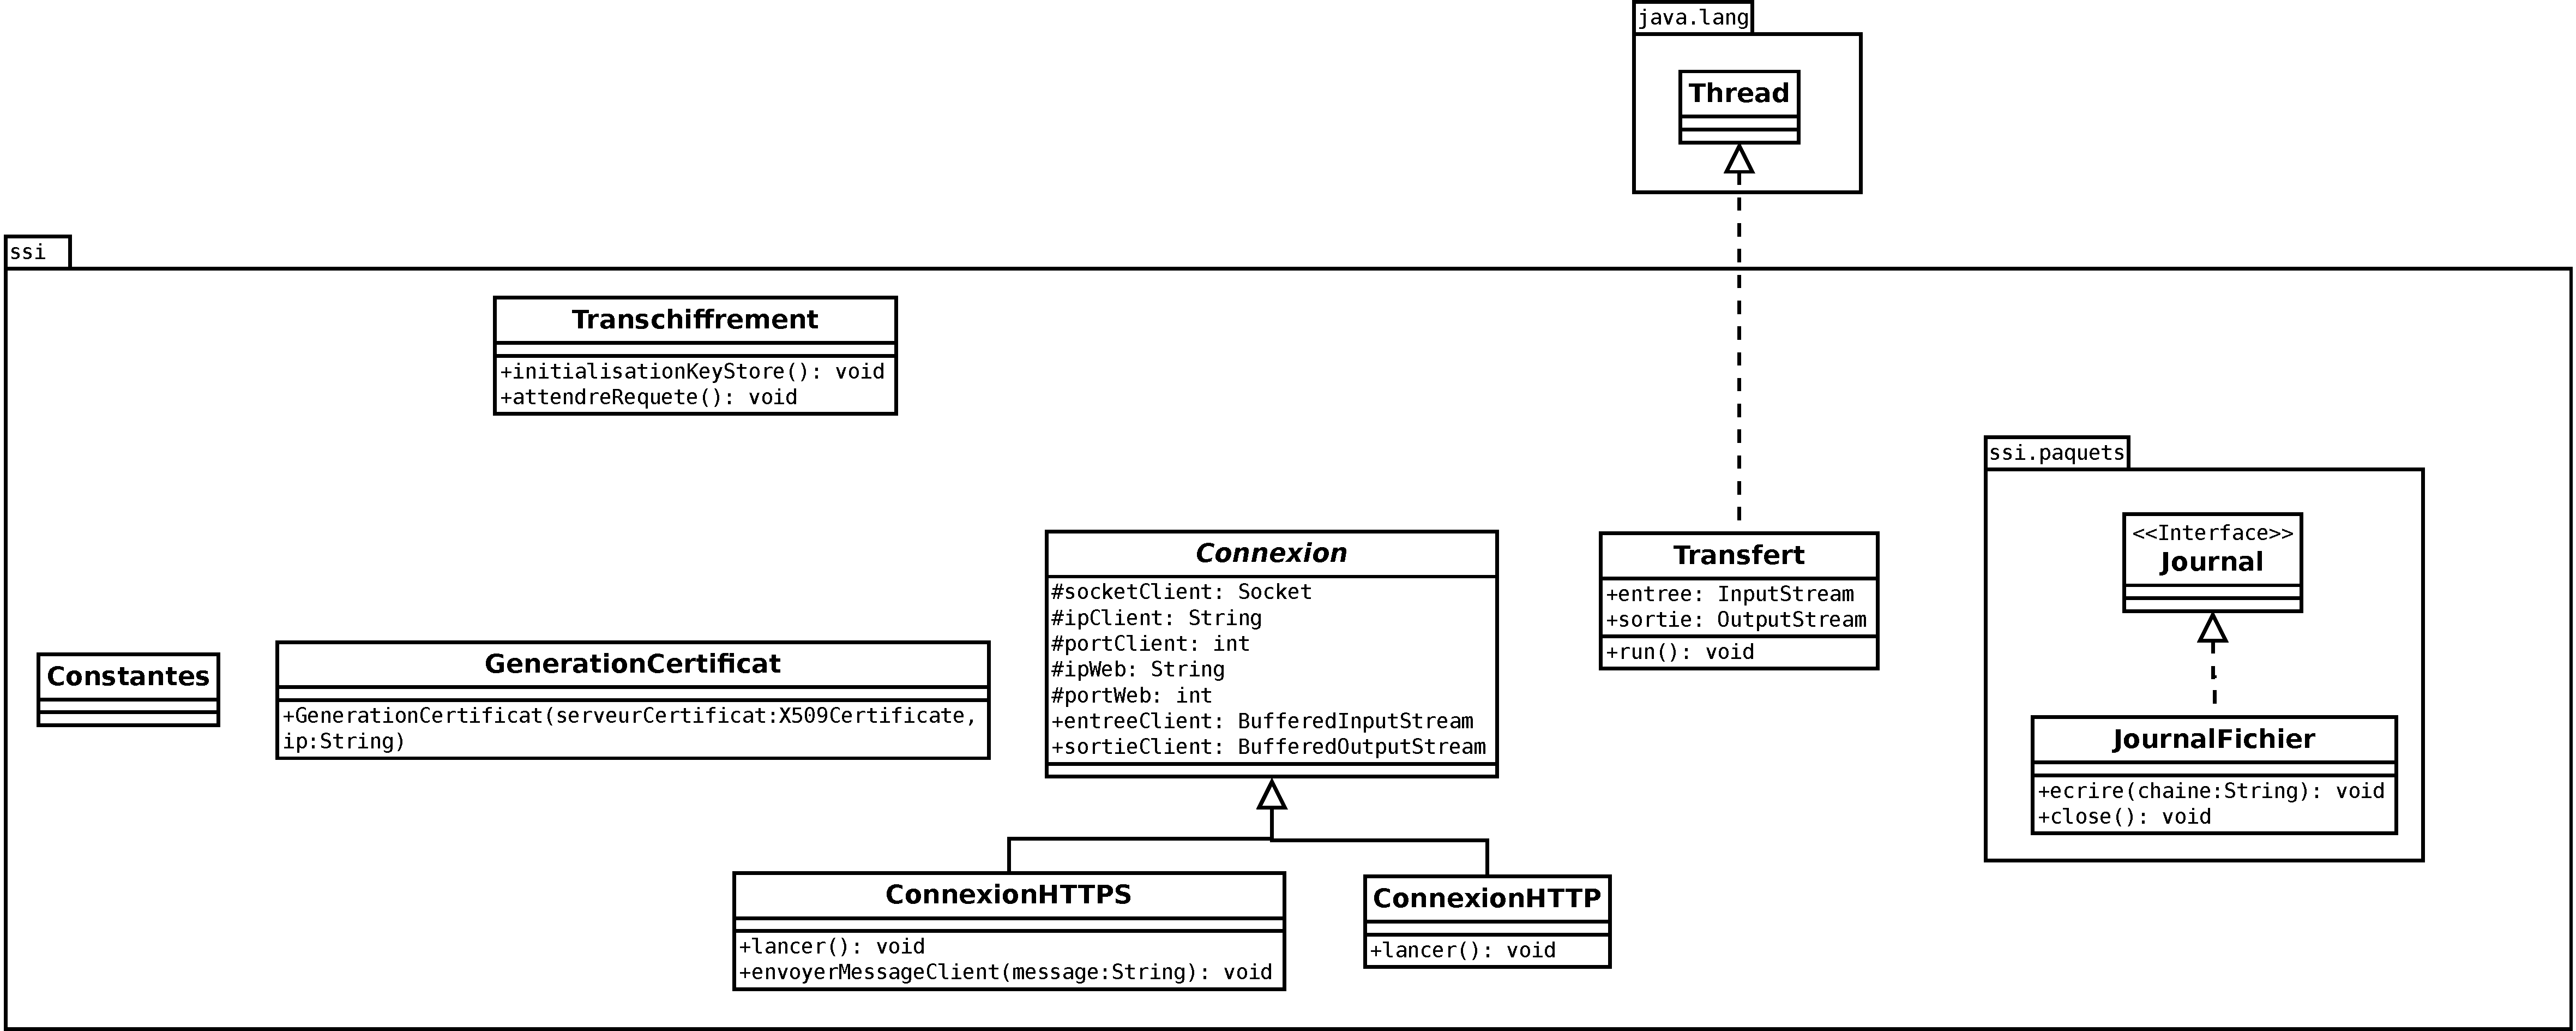
\includegraphics[width=0.8\textwidth]{images/uml.pdf}

\subsubsection*{Implémentation}


\paragraph{Threads}
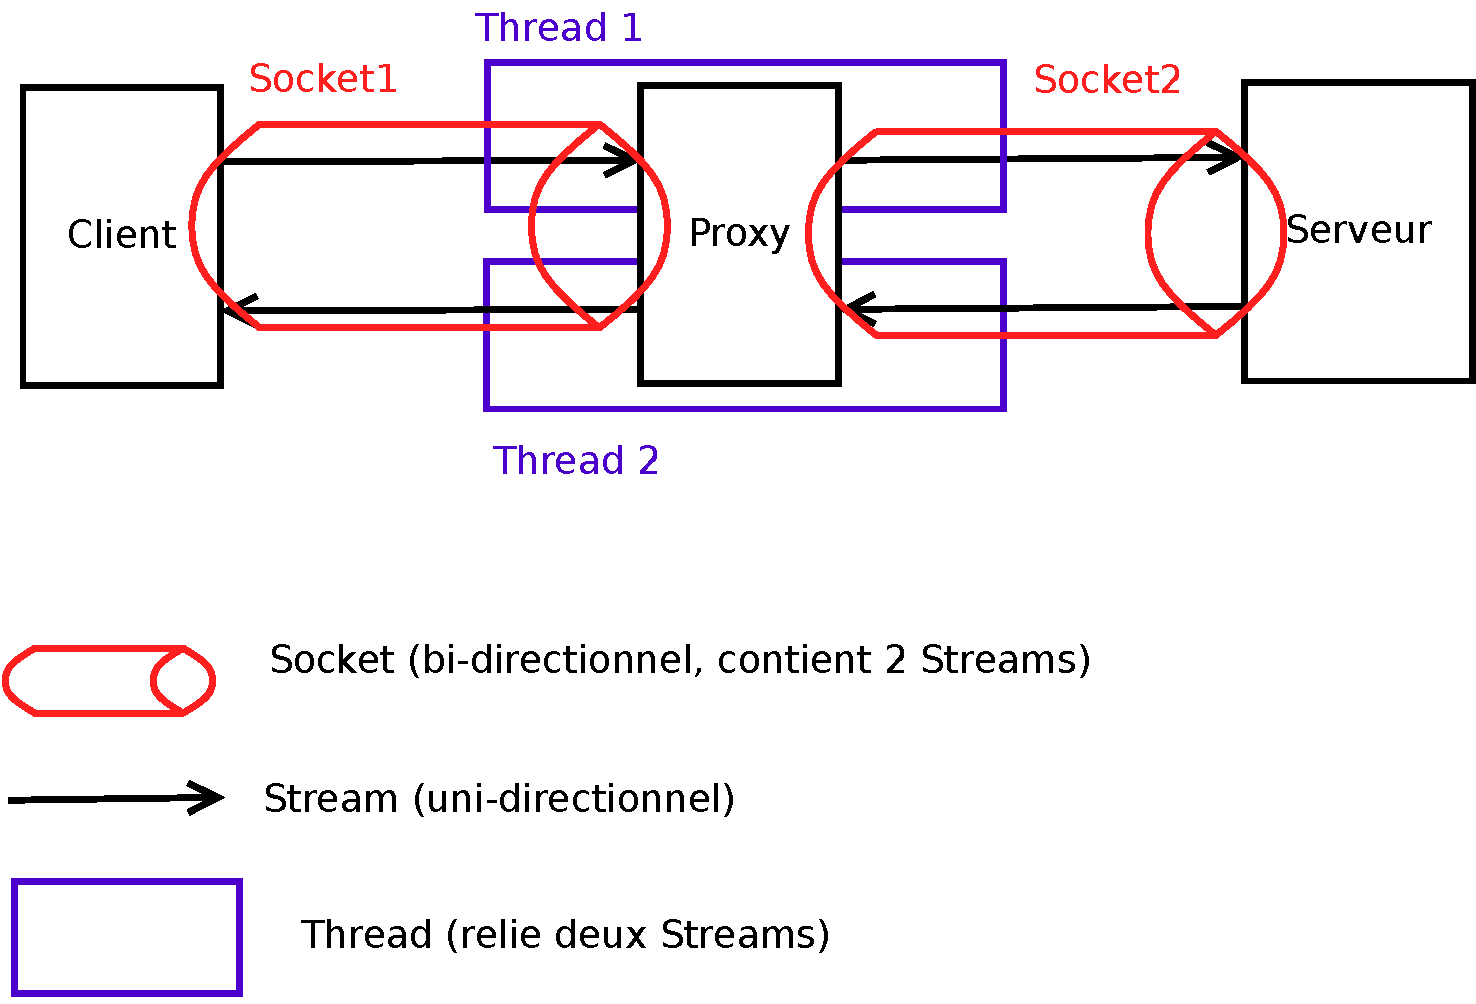
\includegraphics[width=0.8\textwidth]{images/thread.pdf}

\paragraph{Sockets}


\section{Recherche de collision sur des certificats hachés en MD5}

\chapter{Synthèse}

\end{document}
